\begin{figure}[h!]
    \centering
    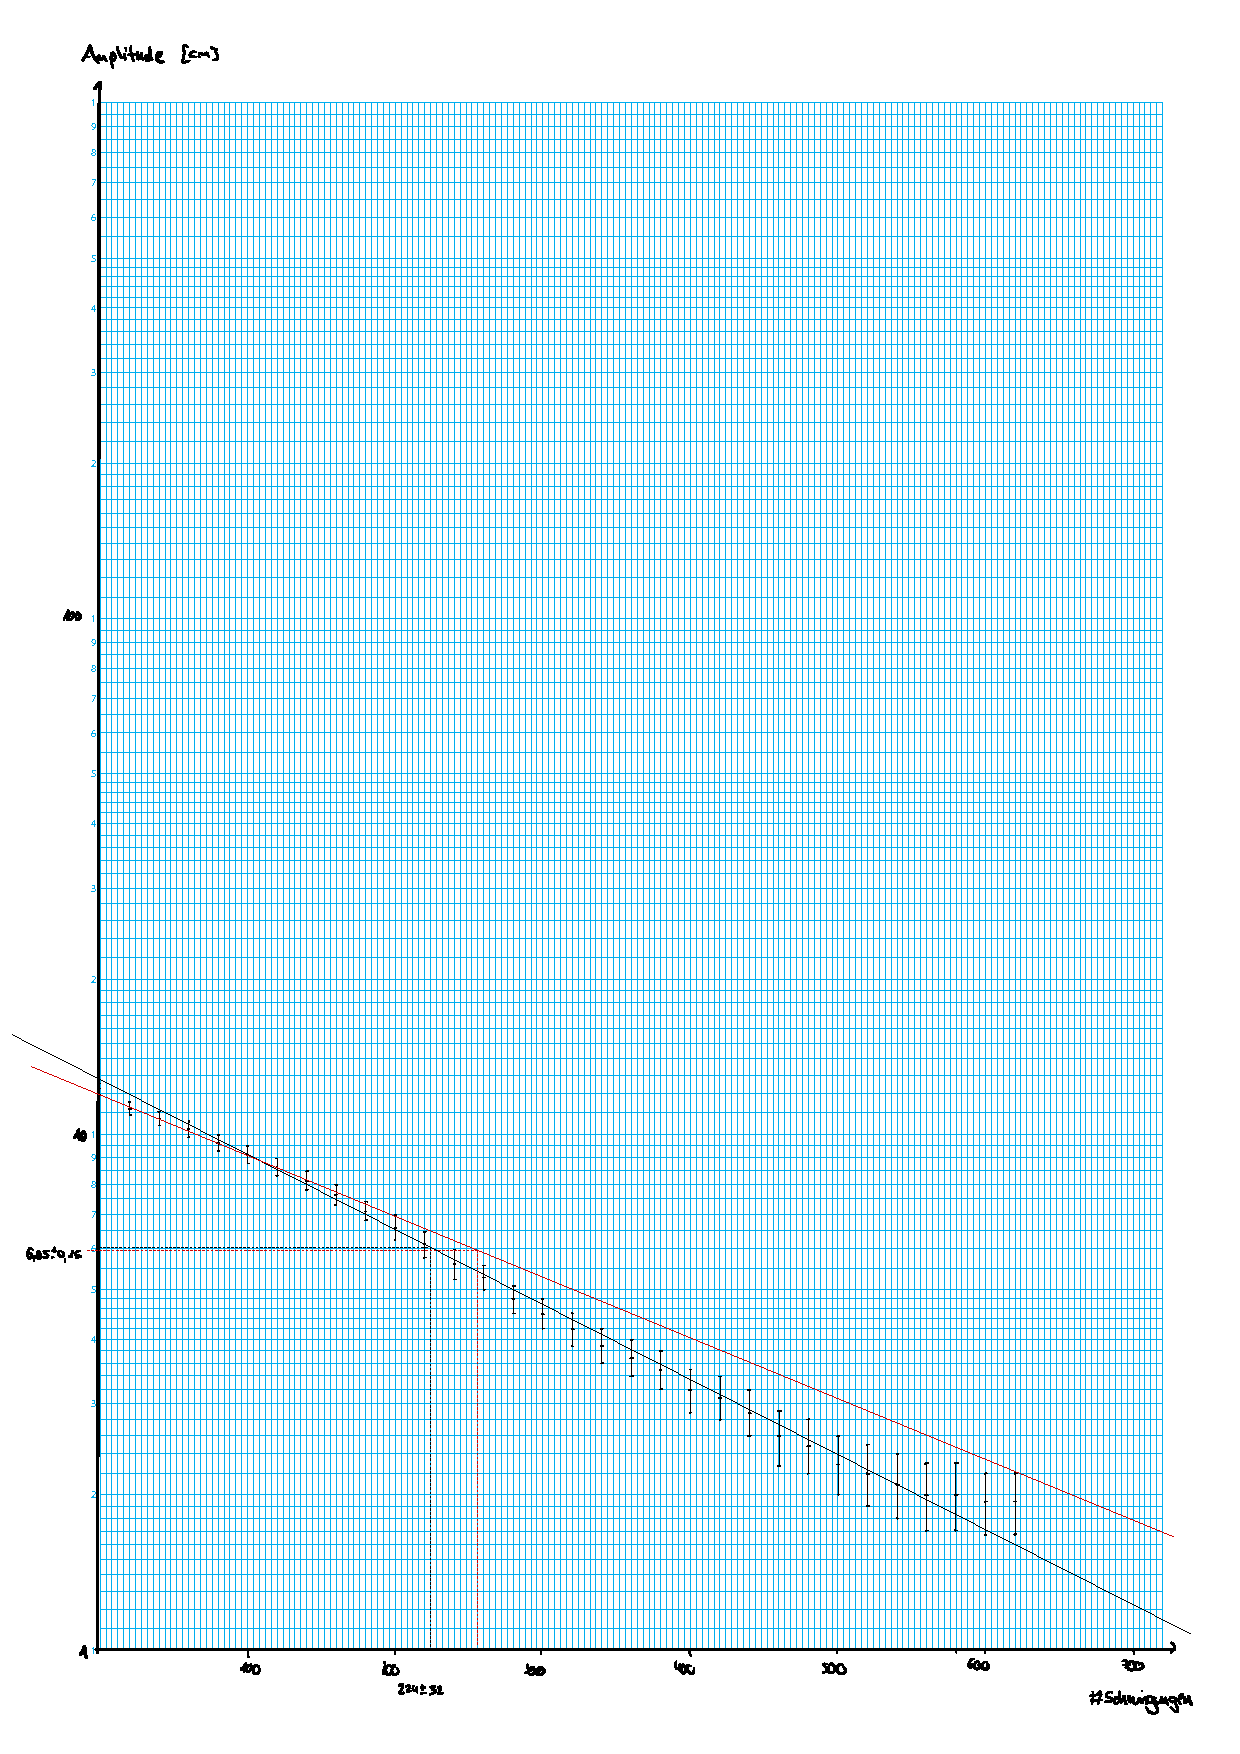
\includegraphics[width = .95 \textwidth]{Dia14.pdf}
    \caption{Diagramm 1}
\end{figure}


\section{Aufgabe I}

Mithilfe der ersten Messreihe wird $g$ nach Gleichung \ref{eq:Tnorm} berechnet.
Dabei gilt für $T_0$ der genauere Fehler von $\Delta T_0 = 0,018\ \text{s}$ als Abweichung des Mittelwerts der fünf Messungen:

\[g =\SI{9,83 \pm 0,13 }{\frac{\meter}{\second^2}}\]

Der Fehler wurde wie folgt berechnet:

\begin{equation}
    \Delta g = 4\pi^2 \sqrt{\left(\frac{\Delta l}{T_0^2}\right)^2 + \left(\frac{2l}{T_0^3}\Delta T_0\right)^2}
\end{equation}

\section{Aufgabe II}

Zuerst wird aus Diagramm 1 die Zahl der Schwingung bei halber maximal Amplitude $n_{1/2}$ bestimmt. 
$t_{1/2}$ kann aus $n_{1/2}$ bestimmt werden durch:
\begin{align}
    t_{1/2} &= n_{1/2} \cdot T_0 \\
    \Delta t_{1/2} &= \Delta n_{1/2} \cdot T_0
\end{align}
Danach lässt sich nach:
\begin{equation}
    \delta = \frac{\ln 2}{t_{1/2}}
\end{equation}

die Dämpfungskonstante $\delta$ bestimmen:

\[ \delta = (1,57 \pm 0,23) \si{\cdot 10^{-3}\frac{1}{\second}}\]

Dabei gilt für den Fehler:
\begin{equation}
    \Delta \delta = \frac{\ln 2}{t_{1/2}^2}\Delta t_{1/2}
\end{equation}



\subsection{Bestimmung der Massen}

Für die Masse allgemein gilt mit $\rho$ als Dichte und $V$ als Volumen:
\begin{equation}
    m = \rho V
\end{equation}
Damit gilt für die Kugel mit $\rho_K$ als Dichte von Eisen:

\[m_k = (176 \pm 8) \si{\gram}\]

Mit dem Fehler:
\begin{equation}
    \Delta m_K = 4\pi r^2 \rho_K
\end{equation}
Und für den Faden genähert als Zylinder mit Höhe $l'$:

\[m_F = (0,2264 \pm 0,0004) \si{\gram}\]

\begin{equation}
    \Delta m_K = \pi r^2 \rho_K
\end{equation}

\subsection{Bestimmung Frquenz ohne Reibung}
Die Eigenfrequenz des Pendels kann nach Gleichung \ref{eq:ho} bestimmt werden mit $\omega_0 = \tfrac{2\pi}{T_0}$. 

\[ \omega_0 = (3,24 ) \si{\Hz} \]

Für $\omega_0$ gilt hier der Wert ohne Dämpfung, da die Größenordnung von $\delta$ in Vergleich vernachlässigbar ist und $\delta$ zusätzlich quadriert wird.
Dementsprechen hat die Dämpfung keinen Einfluss auf $\omega_0$

\subsection{Berechnung $\varphi_0$}
Aus Tabelle 4 kann der Mittelwert der Amplituden mit Fehler bestimmt werden:
\[ \overline{x} = (5,2 \pm 0,6) \si{\cm}\]
Dafür gilt für den Fehler mit Ablesefehler $\Delta a$ und statistischer Abweichung $\sigma$:

\begin{equation}
    \Delta \overline{x} = \sqrt{\sigma^2 + (\Delta a)^2}
\end{equation}

Daraus kann mit Gleichung \ref{eq:phi} $\varphi_0$ berechnet werden.

\[\varphi_0 =( 0,110 \pm 0,006 )\si{\text{rad}}\]

Mit dem Fehler:
\begin{equation}
\Delta \varphi_{0} = 
\sqrt{ \left( \frac{l}{\overline{x}^{2} + l^{2}} \cdot \Delta \overline{x} \right)^{2} 
    + \left( \frac{\overline{x}}{\overline{x^{2} + l^{2}}} \cdot \Delta l \right)^{2} }
\end{equation}

\subsection{Berechnung von $g$}
\begin{itemize}
    \item $T_0 = 1,937435 \si{\second}$
    \item $l = 93,42 \pm 0,12 \si{\cm}$
    \item $r = 1,7500 \pm 0,0125 \si{\cm}$
    \item $m_K \SI{176 \pm 8}{\gram}$
    \item $m_F \SI{0,2264 \pm 0,0004}{\gram}$
    \item $\rho_L = \SI{1,2041}{\cdot 10^{-3} \frac{\gram}{\cm^3}}$
    \item $\rho_K = \SI{7,86}{ \frac{\gram}{\cm^3}}$
    \item $ \varphi_0  = \SI{0,110 \pm 0,006}{\text{rad}}$
\end{itemize}

Abschließen lässt sich daraus unter Berücksichtigung aller Korrekturen die Gravitationsbeschleunigung $g$ mit Gleichung \ref{eq:leckmich} berechnen.

\[\underline{\underline{g = \SI{9,845 \pm 0,014}{\frac{\meter}{\second^2}}}}\]

Dabei gilt für die Fehlerbestimmung:

\begin{align}
\Delta g^{2} 
&= \left( 
    \left( 
        \frac{4\pi^{2}}{T_{0}^{2}}
        \left( 
            1 + \frac{2r^{2}}{5l^{2}} + \frac{\rho_{L}}{\rho_{K}} 
            - \frac{m_{F}}{6m_{K}} + \frac{\delta^{2}}{\omega_{0}^{2}} 
            + \frac{\varphi_{0}^{2}}{8} 
        \right) 
        - \frac{16\pi^{2}r^{2}}{5l^{2}T_{0}^{2}} 
    \right) \cdot \Delta l 
\right)^{2} \\[1ex]
&\quad + \left( 
    \frac{16\pi^{2}lr}{5T_{0}^{2}l^{2}} \cdot \Delta r 
\right)^{2} 
+ \left( 
    \frac{-4\pi^{2}l}{6T_{0}^{2}m_{K}} \cdot \Delta m_{F} 
\right)^{2} \\[1ex]
&\quad + \left( 
    \frac{4\pi^{2}lm_{F}}{6T_{0}^{2}m_{K}^{2}} \cdot \Delta m_{K} 
\right)^{2} 
+ \left( 
    \frac{8\pi l \delta}{T_{0}^{2}\omega_{0}^{2}} \cdot \Delta \delta 
\right)^{2} \\[1ex]
&\quad + \left( 
    \frac{-8\pi^{2}l\delta^{2}}{T_{0}^{2}\omega_{0}^{3}} 
\right)^{2} 
+ \left( 
    \frac{\pi^{2}l\varphi_{0}}{T_{0}^{2}} \cdot \Delta \varphi_{0} 
\right)^{2}
\end{align}
